\section{Protocol compatibility is not agent competence}\label{sec:C19:scope}
An interoperability protocol standardizes messages and declared behavior across process or organizational boundaries. It can make tools discoverable, data addressable, and delegated work trackable. It does not determine whether an agent chooses the right capability, constructs a correct plan, or interprets evidence appropriately. A protocol-conformant system can execute a perfectly well-formed but irrelevant or unauthorized operation if the surrounding application grants it that authority.

MCP and A2A address different boundaries. MCP connects an application host and its clients to servers exposing context and capabilities. A2A represents interactions with a remote agent through messages, tasks, artifacts, and declared capabilities~\cite{mcp2026spec,cumb2026a2aspec101}. A tool server can wrap sophisticated computation, and a remote agent can internally use many tools. The distinction is the contract exposed to the caller, not an ontological test of whether the remote implementation is intelligent.

The literature and implementation review for this chapter is current through 29 October 2026. The current MCP revision identified in the official versioning documentation is 2026-07-28~\cite{mcp2026versioning}. The versioning policy permits backwards-compatible changes while a revision is current, so a dated specification URL alone does not freeze every document; the inspected schema commit is recorded separately. Earlier handshake-based revisions remain historically important, but their session and initialization assumptions must not be presented as the current core protocol. A2A's task lifecycle is anchored to the v1.0.1 repository snapshot~\cite{a2a2026task}; ancillary documentation using a moving ``latest'' URL remains a reproducibility limitation unless archived or pinned independently.

The application must map protocol identities to its own semantic identities. A JSON-RPC request identifier correlates a request and response. It is not automatically a durable task identifier, a user session, or an idempotency key for an external effect. Similarly, a remote agent's declared name is not proof of its authority. Confusing these roles can produce duplicate work, cross-session state mixing, or misplaced trust while every message still validates against a schema.

For technical comparison, define interoperability at several levels: transport connectivity, message-schema compatibility, feature negotiation, semantic agreement about state transitions, authority propagation, and reliable recovery. Passing a connectivity test establishes only the first levels. A useful conformance report should identify which levels were exercised and which remain assumptions. The analysis below separates the current normative message facts from the systems deductions that follow when those messages carry long-running agent work.


% SCIENTIFIC_FIGURE_C19
Figure~\ref{fig:C19:overview} distinguishes request correlation, task lifecycle, and conversational context; none of these identifiers establishes current dispatch authority.
\begin{figure}[!htbp]
\centering
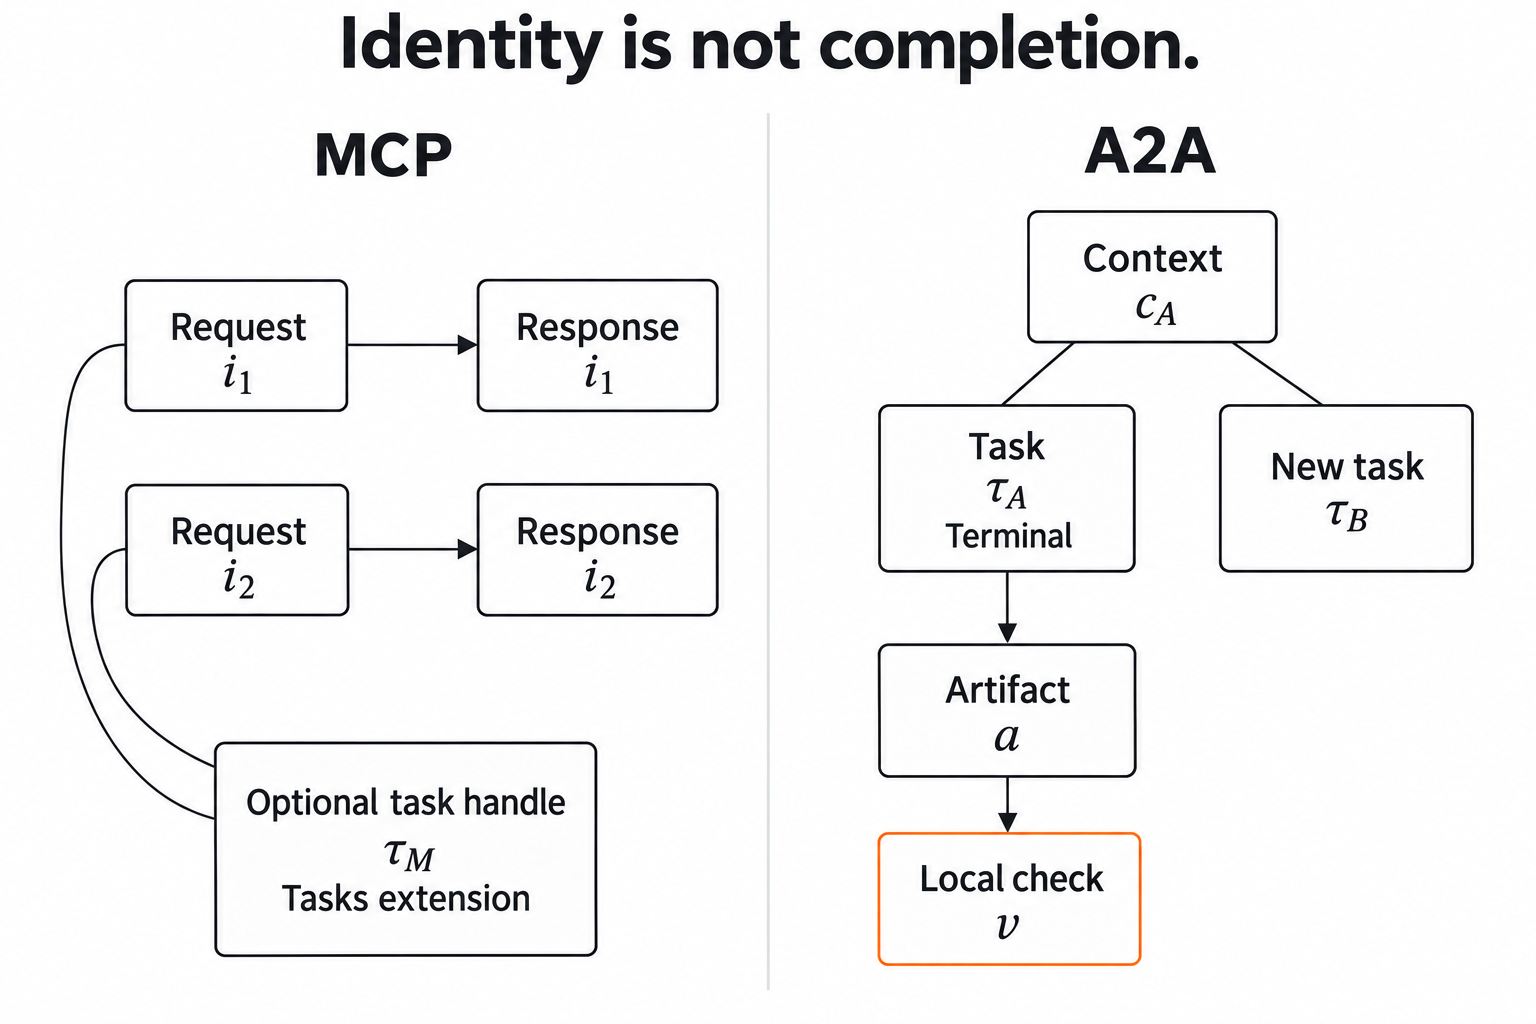
\includegraphics[width=\linewidth]{book/figures/assets/F19review.png}
\caption{Protocol identifiers bind different objects. MCP RPC identifiers correlate individual exchanges; an optional Tasks-extension handle can relate requests to durable work. A2A context identifiers group interactions, while task identifiers bind units of work. A terminal task is not restarted; a later follow-up can create a new task in the same context. Returned artifacts still need local validation. No automatic cross-protocol identity or authority mapping is implied.}
\label{fig:C19:overview}
\end{figure}
